\chapter{Maximum likelihood estimation} \label{mle}
\index{maximum likelihood estimation|ff}
\index{MLE|see{maximum likelihood estimation}}
%@-     so lgrind will play nice with makeindex

Maximum likelihood estimators (MLEs) are the bread and butter of
statistics. Most of the techniques we've handled so far are MLE
techniques, except mathematicians over the ages have found ways to hide
that fact from you. But if there isn't a nice, convenient way to get
around doing the maximization, you'll have to do it yourself. Fortunately,
the GSL has the \cinline{gsl\_multimin} family of objects, to help you find
the optimal parameters. Apophenia even has an \ttind{apop\_maximum\_likelihood}
function that preps and calls the GSL functions for you. You give it a
function and some parameters, and it will find the optimum.


\paragraph{The \ind{log likelihood function}}	\label{the score}
By itself, the PDF is the likelihood that a given value occurs (given
the parameters of the PDF); any of the functions listed in section
\ref{distlist} will do. Define the Log likelihood as $L=\ln f$, the
Score\index{score} as

$$S={\partial \ln f\over \partial \theta}$$ 

and the Information variable\index{information variable} as

\begin{eqnarray}
I&=&-{\partial S \over \partial \theta}			\nonumber\\
&=&-{\partial^2 L \over \partial \theta^2}.		\nonumber
\end{eqnarray}

$L$, $S$, and $I$ will appear over and over again, so we may as well get
to know them. First, due to all that exponentiation in the distributions
of Section \ref{distlist}, $L$ is often much easier to deal with, yet
is equivalent to the PDF for most of our purposes. 

Further, let the probability of observing $X_1$ as it is in our data
set be $p_1$, and the probability of $X_2$ being as observed is $p_2$.
Assuming that $X_1$ and $X_2$ are independently distributed, their
probability is $p_1\cdot p_2$; this is basically the definition of
statistical independence. If we have a thousand observations, then the
probability of observing the data set we have is $\prod_{i=1}^{1000} p_i$.
Since each $p_i\in (0,1]$, this product is probably on the order of
$1\times 10^{-1000}$. This is a delicate number, and details of
implementation in hardware could easily break it; this is what computer
scientists call an {\sl underflow error}. Taking logs, each value of
$p_i$ is now a negative number, e.g., $\ln(0.5)\approx -0.69$ and $\ln(0.1)\approx -2.3$.
But the product above is now a sum:
$$\ln\left[\prod_{i=1}^{1000} p_i\right] = \sum_{i=1}^{1000} \ln(p_i).$$
Thus, the log likelihood of our typical data set is on the order of
-1000 instead of $1\times 10^{-1000}$---much more robust and manageable.

The second benefit to using the log likelihood is analytic: since $S \cdot f = {\partial f
\over \partial \theta}$, the derivative of the expectation in terms of
$\theta$ can be rewritten as the expectation of $S$.\footnote{%
	Note the sleight of hand: the derivative of the expectation is
	${d\over d\theta}\int f dy$; while we want $\int {d f\over
	d\theta} dy=\int S \cdot f dy$ [Note how this means $E(S)=0$, by the
	way, since the integral of the pdf is one, and $d1/d\theta=0$].
	If we can't reverse the integral and derivative like this, none
	of this applies. But we can in the case of any exponential
	family. You can look that up, but here, we can rest assured that
	the Normal, Gamma, Beta, Binomial, Poisson, \&c. are all in this
	family.} 

There are some fun tricks you can do with these functions, most of which I'll have to
skip over.  The neat trick most worth mentioning is the \ind{information equality}, that
$E(I)=\var(S)$, which you can prove by calculating ${\partial E(L)\over
\partial \theta}$.

\section{Why likelihood functions are great} There are two reasons, with four names.

\paragraph{MLEs achieve the Cramer-Rao lower bound} 
        \index{Cramer-Rao Inequality}		\label{cr} 
Say we have an unbiased estimator of $\theta$,
$\hat\theta(y_1,\dots,y_n)$. Cramer \& Rao say:
\begin{eqnarray}
\var(\hat\theta)&\geq&(n \var(S))^{-1}		\nonumber\\
		&=&\left(nE\left({\partial^2 L\over \partial
\theta^2}\right)\right)^{-1}			\label{CRLB}
\nonumber\end{eqnarray}

\comment{
A sketch of the proof: Take my word for it that $E(\hat\theta
\overline S)={1\over n}$. Since $\overline S=0$, that's equivalent to
$\cov(\hat\theta, \overline S)={1\over n}$.  Plug that into Cauchy-Schwarz:
$\var(\hat\theta)\var(\overline S)\geq {1\over n^2}$. Plug
$\var(S)=n\var(\overline S)$ in to that, and the first line of the above
drops out\cite{goldberger}. The second line uses the information
equality from above.
	}
Just remember: the Cramer-Rao lower bound is the inverse of the expectation of the
derivative of the derivative of the log of the likelihood function.

The Cramer-Rao lower bound is
called a `lower bound' because Mr.s Cramer and Rao proved that any
estimator of $\beta$ must have a variance greater than or equal to the
CRLB. Your favorite probability textbook (e.g., \cite{casella:berger})
will also prove that for the MLE, the variance is actually equal to the
CRLB, meaning that we can not get an estimator of $\beta$ which will
have a smaller variance.

\paragraph{The Neyman-Pearson lemma} There are two types of error we could
have with a hypothesis test: Type I is that we reject the null when it's
true; Type II is that we accept the null when it's false. The first type
is the one we focus on; it's what we mean when we say that our
test has $\alpha=95\%$ confidence. What about Type II errors? Well,
Neyman and Pearson showed that a likelihood ratio test will have the
minimum possible Type II error of any test with the $\alpha$ that we
selected. After establishing this fact, we just ignore Type II errors.

\section{Description: Maximum likelihood estimators} 


Estimating an existing model via maximum likelihood estimation simply requires 
filling out a form describing your preferences and then calling the model's \cinline{estimate} method.
The form in question is a \ttind{apop\_estimation\_params} structure, that
describes the method, the starting point, the step size, and the
tolerance.
For example:
\begin{lstlisting}
apop_estimation_params *ep  = malloc(sizeof(apop_estimation_params);
double  starting_point[2]   = {1,1};
ep->method      = 000;
ep->step_size   = 1e-1;
ep->tolerance   = 1e-5;
ep->verbose     = 1;
ep->starting_pt = starting_point;
apop_gamma.estimate(my_data, an_inventory, ep)
\end{lstlisting}

Here are the parts to the  \ttind{apop\_estimation\_params}
structure you need to set. 

\paragraph{The method} There are currently four you can choose from.
[Also, there are two more that  just aren't hooked in yet. If you're
comfortable exploring the internals of Apophenia, have a look at the
\cinline{wnbridge.c} file.]


\begin{itemize}
\item {\bf 000: The Nelder-Mead simplex algorithm} Draws a polygon and then attempts to shift the corners of the polygon.
\item {\bf 100: conjugate gradient (Fletcher-Reeves)} This is the
default. Basically, we take the derivative in all directions and find
the linear combination of these directions that indicates the fastest
climb. Clearly, this depends on knowing derivatives; see below.
\item {\bf 200: conjugate gradient (BFGS: Broyden-Fletcher-Goldfarb-Shanno)}  Another conjugate gradient method, that calculates the direction of travel differently. See \cite{avriel:nonlinear} for definitions of all of these methods.
\item {\bf 300: conjugate gradient (Polak-Ribiere)} Yet another conjugate gradient method.
\end{itemize}

As a practical matter, your best bet is to either just go with the default (Fletcher-Reeves) or try them all using a tournament as described below. 
If you expect the derivatives to be perverse, then you may want to try the derivative-free simplex algorithm.

There is also the question of how the gradients are calculated. If
analytic gradients are available, then those are probably preferable, but
Apophenia will automatically calculate numerical gradients as necessary.
Since the variance of an MLE is the Cramer-Rao lower bound, we will use
the gradients to calculate the variance, so even when using a
derivative-free simplex algorithm, the variance will still be using
gradients, somehow derived.

Just in case the analytic gradients don't work out for you, there is a
means of just using the numeric gradients. This is primarily useful for debugging:

\begin{itemize}
\item 0: If (and only if) no gradient is available, use numerical approximations.  (default)
\item 1: Use numerical approximations even if an explicit dlog likelihood is given. 
\end{itemize}

The actual method you give is the sum of the method type above plus the
gradient handling method. Thus the default is equal to 100, for example, and the
Nelder-Mead simplex algorithm forcing numerical derivatives would be
001.\footnote{Yes, 000 reduces to 0 and 001 reduces to 1. The internals
don't care, so use whichever form makes the most sense to you as a human.}


\paragraph{The step size} This is the initial distance that the
algorithm will use to start searching for points. Basically arbitrary
because all of these algorithms are adaptive, meaning that they will
change the step size as they see fit.

\paragraph{Tolerance} The algorithm will basically stop when it feels
that the calculated log likelihood is changing by less than this amount,
indicating that the search is at a local maximum and the first derivative of
the log likelihood function is nearing zero.

\paragraph{Verbose} Should the search output the points it is evaluating?
This is useful for long evaluations to reassure you that nothing is
broken; for example, some of the GSL's searches can get into two-step loops.
It is probably a good idea to run your search verbosely at least once.
Also, see \cinline{apop\_opts.mle\_trace\_path} below.

\paragraph{Starting point} an array of doubles indicating where you want
your search to begin. Being an array, you can use a form like the above
to initialize it (but then it will be destroyed when you leave the
function that it was initialized in---remember this if you want to
access the starting point in the estimate that the MLE outputs).


\subsection{Restarting} One convenient trick is to solve for an MLE and
then restart the procedure at the point where the first MLE found its solution.
To do this, use \ttind{apop\_estimate\_restart}.

The function takes three arguments: a prior estimate that you have
already calculated, a method, and a scaling factor. 

First, the function copies off the \cinline{apop\_estimation\_params}
from the \cinline{apop\_estimate} sent in, and then makes a series of
modifications.  If the new method sent in is -1, then the new MLE will
use the same method as before; otherwise specify one of the methods
listed above. The step size and the tolerance are both multiplied by the
scaling factor sent in (so if this is 1, no change is made). If the
estimated parameters for the original estimate is finite and bounded, then 
the starting point in the new \cinline{apop\_estimation\_params}
structure is set to the estimated value; if some element of the
estimated parameters are infinity or NaN, then the original starting
point is reused.

Then, the ML estimation is run again, and we now have two estimates: the
original and the new one. If the new one has not-finite or NaN values,
then it is thrown out and the original returned. If the new estimate 
has a higher log likelihood, then it is returned, and the old estimate
is deleted.  The less likely estimate (which may be the one you sent in) is freed. That is,
there is no memory leak when you run a tournament like:
\begin{lstlisting}
est = apop_estimate_restart(est, 200, 1);
est = apop_estimate_restart(est, 100, 1e-2);
est = apop_estimate_restart(est, -1, 1e-2);
\end{lstlisting}
The estimate can only get better every time you run
\ttind{apop\_estimate\_restart}, so the only cost to running a lengthy
tournament is your time waiting for the estimates to converge.

\subsection{Graphing the path} All of the methods above consist of
trying a series of candidate points. 
If \index{apop\_opts!mle\_trace\_path@\cinline{mle\_trace\_path}}\cinline{apop\_opts.mle\_trace\_path}
has a name of positive
length, then every time the MLE evaluates the function, then the value
will be output to a table in the database with the given name. You can
then plot this table to get an idea of the path the estimation routine
used to arrive at its MLE.

First, set this variable and run the MLE. The begin/commit wrapper
speeds things up a touch, but this will clearly be slower than without
taking notes:
\begin{lstlisting}
    strcpy(apop_opts.mle_trace_path, "path");
    apop_query("begin;");
    e   = apop_zipf.estimate(...);
    apop_query("commit;");
\end{lstlisting}
Then, plot using a function like the below. Notice that you will want
\cinline{splot} for 3-d variables and \cinline{plot} for 2-d. The change in width
and pointsize is to remind the eye that the lines connecting the points
only indicate the path the maximizer went along, not actual values of
the function.
\begin{lstlisting}
static void plotme(char *outfile){
FILE            *f;
gsl_matrix      *traced_path;
    f       = fopen(outfile, "w");  //overwrites. Use "a" to append.
    fprintf(f,"splot '-' with linespoints linewidth 0.5 pointsize 2\n");
    traced_path = apop_query_to_matrix("select * from %s"
                                        , apop_opts.mle_trace_path);
    fclose(f);
    apop_matrix_print(traced_path, "\t", outfile);
}
\end{lstlisting}

Finally, call \ind{Gnuplot} from your command line:
\begin{lstlisting}
$ gnuplot -persist < plotme
 (or)
$ gnuplot plotme -
\end{lstlisting}

\begin{figure}
\scalebox{0.4}{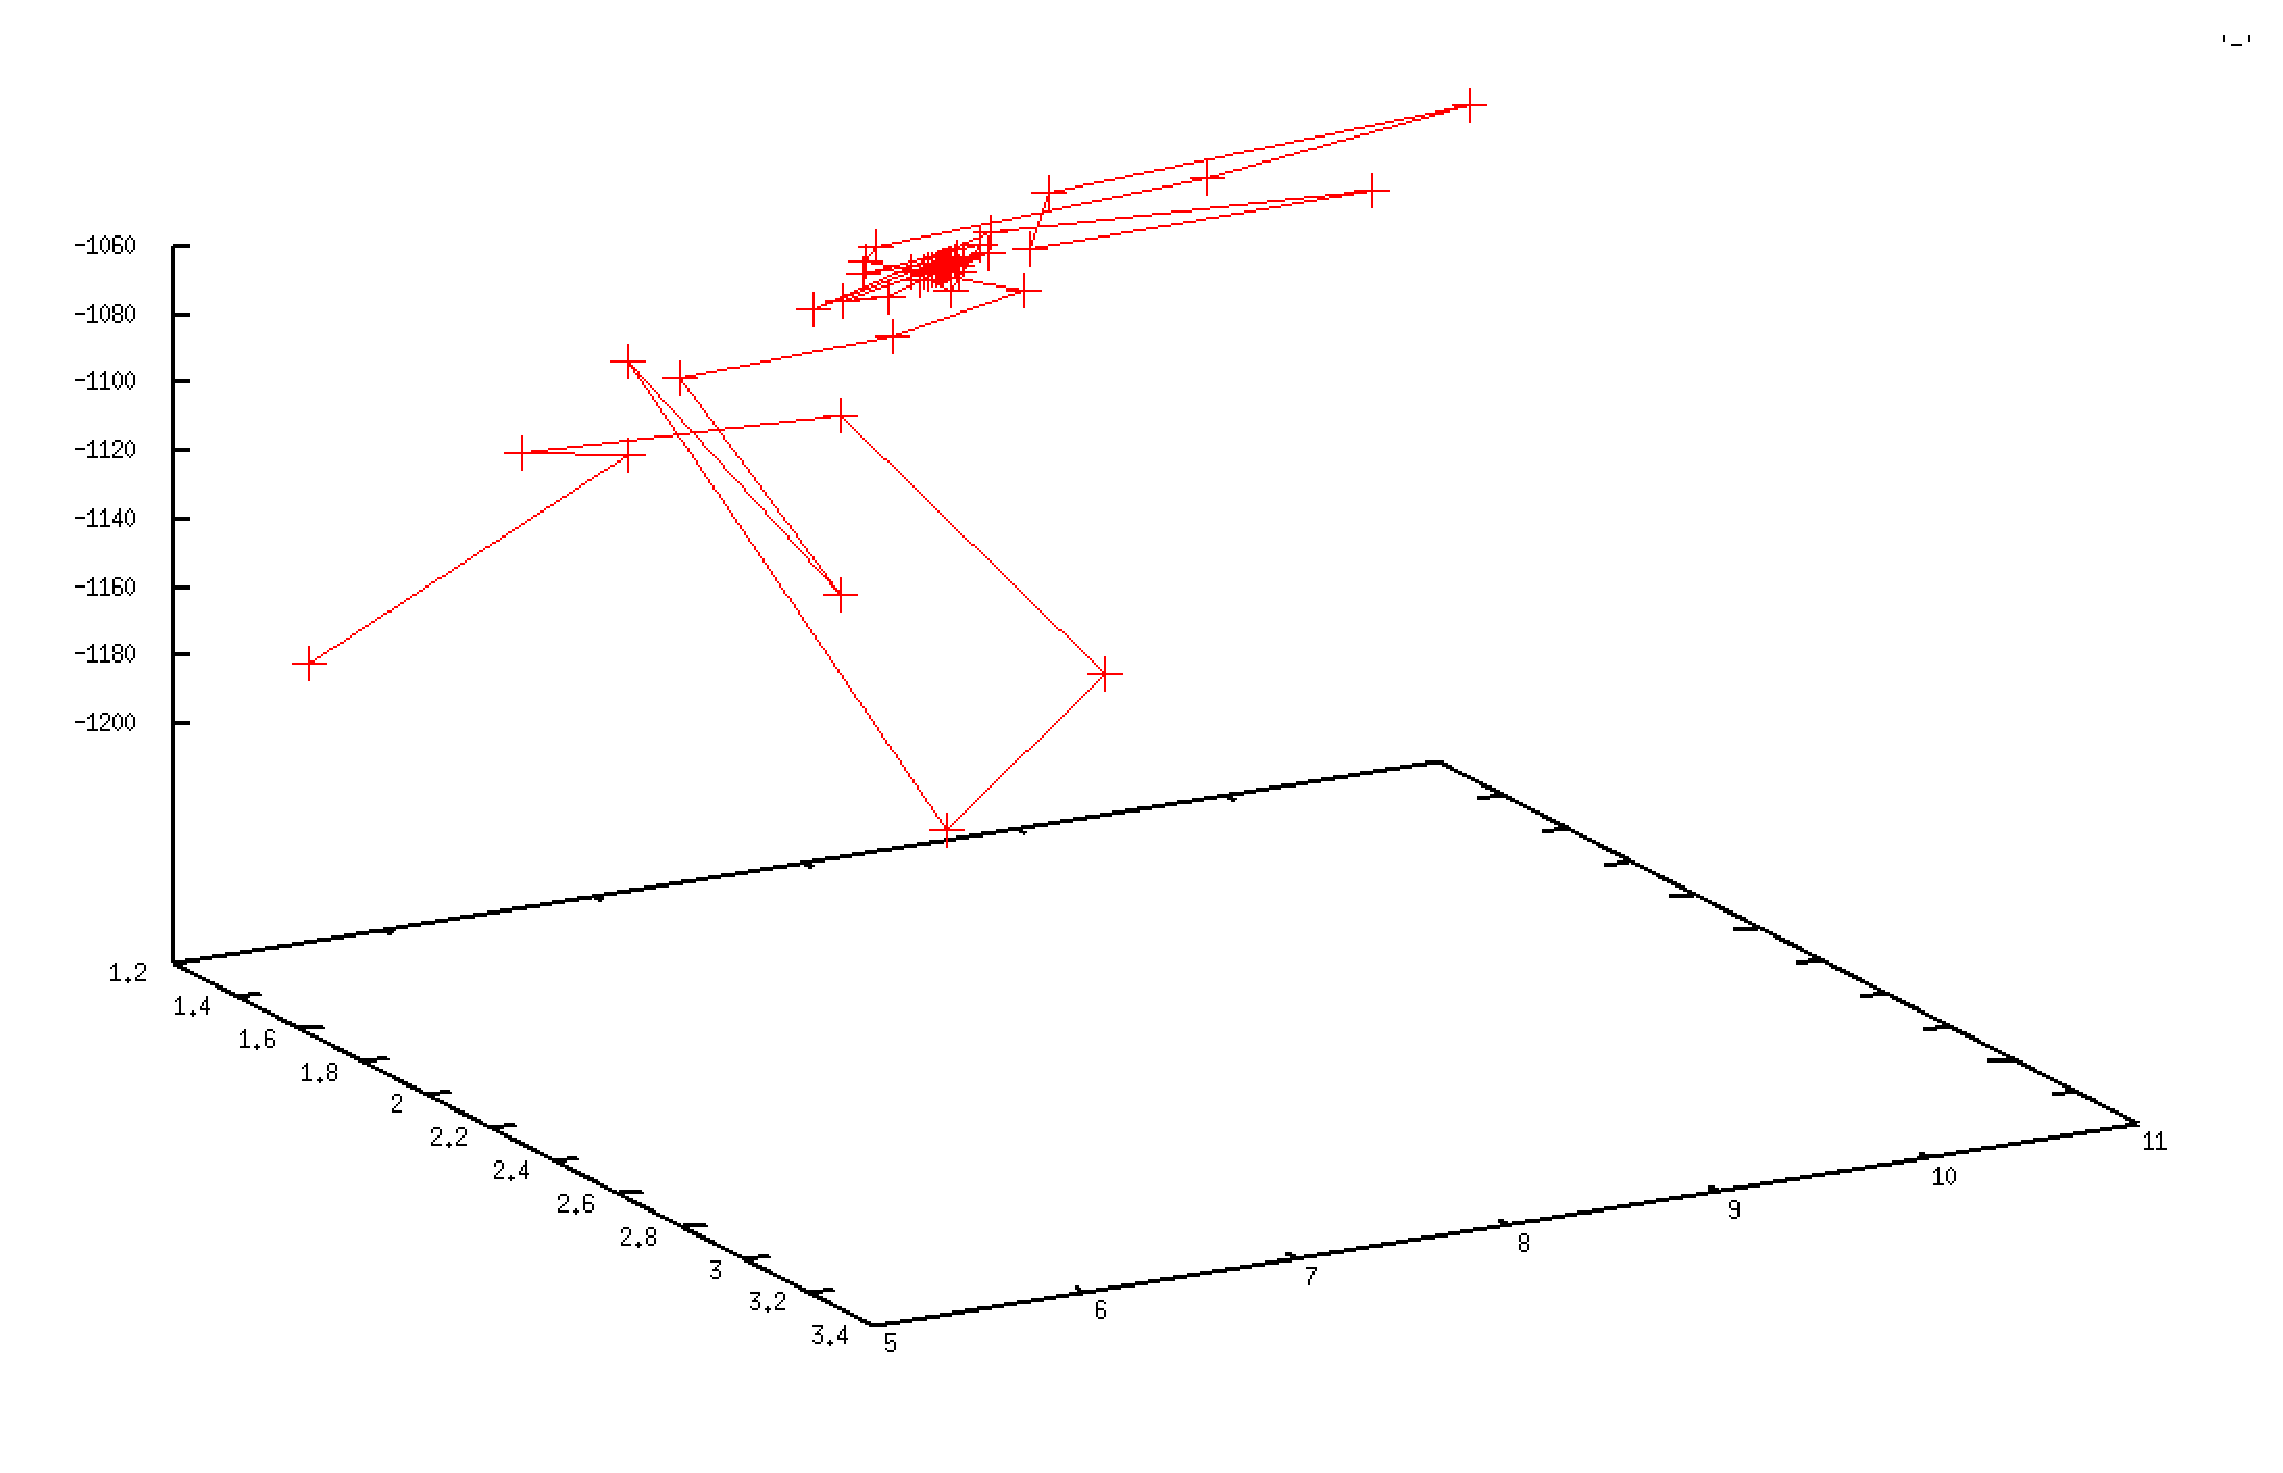
\includegraphics{search}}
\caption{A search for an optimum using a conjugate gradient method.}
\end{figure}

\section{Hypothesis testing: Likelihood ratio tests} Every test
in the last chapter was a likelihood ratio test---I just didn't tell
you what the likelihood function was. Those functions are easy because
they've been carefully studied and methods have been found to let you
calculate them without explicitly writing down a likelihood function
and calculating its value at various locations.

But if your data is at all interesting, then you'll need to write down
the likelihood function yourself.  Fortunately, we have a computer to
do the tedious math, unlike poor Mr. Gauss, who had no such conveniences.
Also, we have the Cramer-Rao lower bound to tell us what the variances
are. 

[...]


\section{Writing your own}
The design of the \cinline{apop\_model} hopes to make it as easy as possible for you,
dear reader, to write new models. For the most part, all you need to
do is write a log likelihood function, and \ttind{apop\_maximum\_likelihood}
does the rest. The steps:


\begin{itemize}
\item Write a likelihood function. Its header will look like this:
\begin{lstlisting}
double apop_new_log_likelihood(const gsl_vector *beta, void *d)
\end{lstlisting}
where \cinline{beta} will be the parameters to be maximized, and \cinline{d} is the fixed parameters---the data. In every case currently included
with Apophenia, \cinline{d} is a \cinline{gsl\_matrix,} but you do not have to conform
to that. This function will return the value of the log likelihood function at the given parameters.

\item Is this a constrained optimization? See section
\ref{constraintwriting} on how to write a constraint function.

\item Write the \cinline{estimate} method, so users can call 
\cinline{apop\_new\_likelihood.estimate(...)}. For an MLE, this will be one line,
as follows:
\begin{lstlisting}
static apop_estimate * new_estimate(apop_data * data, 
                        apop_inventory *uses, void *parameters){
    return apop_maximum_likelihood(data, uses, 
                            apop_new_log_likelihood, parameters);
}
\end{lstlisting}
By using the \ttind{static} keyword, the function name will only be
known to this file, so you can name it what you wish.  But since you
will be putting a pointer to the function into an object below, you
can use the above-mentioned 
\cinline{apop\_new\_likelihood.estimate(...)}
form to call this function. You may want to type all of the functions in
your new model as \cinline{static}.


\item Write the object. In your header file, include 
\begin{lstlisting}
apop_model apop_new_likelihood = {"The Me distribution", 
            number_of_parameters, 
{       //what will apop_new_likelihood.estimate return?
        1,      //parameters 
        1,      //covariance
        1,      //confidence
        0,      //predicted
        0,      //residuals
        1,      //log_likelihood
        1       //names;
},          new_estimate,
            new_log_likelihood, 
            NULL,   //place dlog likelihood here.
            NULL,   //place constraint fn here.
            NULL    //place RNG here.
            };
\end{lstlisting}
If there are constraints, then replace the appropriate \cinline{NULL} with the right constraint function; see below.
\cinline{number\_of\_parameters} is probably a positive integer like \cinline{2}, but
it is often (the number of columns in your data set) -1, in which case,
set \cinline{number\_of\_parameters} to \cinline{-1}.

\item Test. Debug. Retest.

\item Optional: write a gradient for the log likelihood function. This
typically involves calculating a derivative by hand, which is an easy
problem in high-school calculus. The function's header will look like: 
\begin{lstlisting}
void apop_new_dlog_likelihood(const gsl_vector *beta, void *d, 
                                    gsl_vector *gradient)
\end{lstlisting}
where \cinline{beta} and \cinline{d} are fixed as above, and \cinline{gradient} is a \cinline{gsl\_vector} with dimension matching \cinline{beta}. 
At the end of this function, you will have to assign the appropriate derivative to every element of the gradient vector:
\begin{lstlisting}
gsl_vector_set(gradient,0, d_a);
gsl_vector_set(gradient,1, d_b);
\end{lstlisting}
Now add the resulting dlog likelihood function to your object, by replacing the \cinline{NULL} labeled "place dlog likelihood here" with the name of your dlog likelihood function.
\item Send the code to the maintainer for inclusion in future versions of Apophenia.
\end{itemize}


\subsection{Setting
constraints}\index{optimization!constrained}\label{constraintwriting}

The problem is that the parameters of a function must not take on
certain values, either because the function is undefined for those
values or because parameters with certain values would not fit the
real-world problem.

The solution is to rewrite the function being maximized such that the
function is continuous at the constraint boundary but takes a steep
downward slope. The unconstrained maximization routines will be able
to search a continuous function but will never return a solution that
falls beyond the parameter limits.

If you give it a likelihood function with no regard to constraints plus
an array of constraints, \ttind{apop\_maximum\_likelihood} will combine
them to a function that fits the above description and search accordingly.

This is similar to the common penalty function methods of turning an
constrained problem into an unconstrained one, as in \cite{avriel:nonlinear},
with a few differences. Primarily, we don't know if the constraint is
because the author of the system declared an arbitrary cutoff (`we can't spend more
than \$1,000.') or if evaluating the likelihood function fails
($\ln(-1)$). 

A constraint function must do three things:
\begin{itemize}
\item It must check the constraint, and if the constraint does not bind (i.e., the parameter values are OK), then it must return zero.
\item If the constraint does bind, it must return a penalty, that indicates how far off the parameter is from meeting the constraint.
\item if the constraint does bind, it must set a return vector that the likelihood function can take as a valid input. The penalty at this returned value must be zero.
\end{itemize}

The idea is that if the constraint returns zero, the log likelihood
function will return the log likelihood as usual, and if not, it will
return the log likelihood at the constraint's return vector minus the
penalty. To give a concrete example, here is a constraint function that
will ensure that both parameters of a two-dimensional input are both
greater than zero:

\begin{lstlisting}
static double beta_zero_and_one_greater_than_x_constraint(gsl_vector *beta, 
                                    void * d, gsl_vector *returned_beta){
double          limit0          = 0,
                limit1          = 0,
                tolerance       = 1e-3; // or try GSL_EPSILON_DOUBLE
double          beta0   = gsl_vector_get(beta, 0),
                beta1   = gsl_vector_get(beta, 1);
        if (beta0 > limit0 && beta1 > limit1)
                return 0;
        //else create a valid return vector and return a penalty.
        gsl_vector_set(returned_beta, 0, GSL_MAX(limit0 + tolerance, beta0)); 
        gsl_vector_set(returned_beta, 1, GSL_MAX(limit1 + tolerance, beta1));
        return GSL_MAX(limit0 + tolerance - beta0, 0) 
                        + GSL_MAX(limit1 + tolerance - beta1, 0); 
}
\end{lstlisting}

Observe how it manages all three of the above steps. First, it checks
the constraints and quickly returns zero if none of them bind. Then, if
they do bind, it sets the return vector to just inside the constrained
region. Finally, it returns the distance (on the Manhattan metric)
between the input point and the point returned. The hope is that the
evaluation system will repeatedly try points closer and closer to the
zero-penalty point, and the penalty will continuously decline as we
approach that point.

For another example, have a look at the budget constraint in the code
listing at the end of this chapter.

\section{Non-stats modeling}    \label{econ101}

The MLE functions of Apophenia are designed to maximize a function
subject to constraints---which sounds a lot like any of a variety of
other problems, especially in Economics. With little abuse of the package,
one could use it to solve non-statistical models involving maximization
subject to constraints. For example, the code listing at the end of this
chapter shows how one could numerically solve a utility maximization
problem from Econ 101. 

It requires a few digressions from the MLE nomenclature:
\begin{itemize}
\item The log likelihood is actually the utility function. Don't take logs,
since that would mess up the marginal utilities.

\item The data is the fixed input to the MLE, which means the parameters:
prices, budget info, utility parameters.

\item The betas in the MLE framework are the free parameters to be
maximized, which in this case means the goods the consumer is choosing.
\end{itemize}

Utility is $U = x_1^\alpha * x_2^\beta$. 
The budget constraint dictates that $P_1 x_1 + P_2 x_2 <= B$.
                                                             
The data vector looks like this:\\
0:  price0\\
1:  price1\\
2:  budget \\
3:  alpha  \\
4:  beta   
                                                             
Most of the work is in writing down all the constraints, since the
function itself is trivial. Having written down the model, the estimation
is one function call, and calculating the marginal values is one more.
Overall, the program is overkill for a problem that can be solved via
two derivatives, but the same framework can be used for problems with no
analytic solutions (to give one example, if the consumer has a stochastic
utility function).


\begin{lstlisting}
#include <apophenia/headers.h>

apop_model econ_101;

static apop_estimate * econ101_estimate(apop_data * dummy, 
                            apop_inventory *uses, void *parameters){
apop_estimate           *est;
apop_estimation_params  mle_params;
apop_data               *p  = apop_data_from_vector(parameters);
    mle_params.method       = 000;
    mle_params.starting_pt  = NULL;
    mle_params.step_size    = 1e-1;
    mle_params.tolerance    = 1e-8;
    mle_params.verbose      = 0;
    apop_inventory_filter(uses, econ_101.inventory_filter);
    est = apop_maximum_likelihood(p, uses, econ_101, &mle_params);
    est->uses.covariance    = 0;    //MLE finds them, but it's meaningless.
    est->uses.confidence    = 0;    //MLE finds them, but it's meaningless.
    est->uses.log_likelihood  = 0;
    return est;
}
%*
// The constraint function, including three constraints: x0>0, x1>0, and
// the bundle is under budget.  First, we check wether anything binds,
// and if not we return zero immediately.  Both sets of constraints are
// handled in the same way: derive new values that are within bounds,
// and report how far you had to move.

static double budget_constraint(gsl_vector *beta, void * d, 
                                        gsl_vector *returned_beta){
gsl_matrix   *budget = d;
double  price0      = gsl_matrix_get(budget, 0, 0),
        price1      = gsl_matrix_get(budget, 1, 0),
        cash        = gsl_matrix_get(budget, 2, 0),
        x0          = gsl_vector_get(beta, 0),
        x1          = gsl_vector_get(beta, 1),
        tolerance   = 1e-3,
        new_x0, new_x1, penalty;
    if ((x0 * price0 + x1 * price1<= cash) && (x0 > 0) && (x1 > 0))
        return 0;
    //else:
    if (x0 <= 0 || x1 <= 0){
        new_x0  = (new_x0 > 0)? x0 : tolerance;
        new_x1  = (new_x1 > 0)? x1 : tolerance;
        penalty = (fabs(new_x0 - x0) + fabs(new_x1 + x1));
    } else {
        new_x0  = GSL_MAX(0, cash - x1* price1);
        new_x1  = GSL_MIN(x1, cash - new_x0* price0);
        penalty = (GSL_MAX(0,x0 * price0 + x1 * price1- cash));
    }
    gsl_vector_set(returned_beta, 0, new_x0);
    gsl_vector_set(returned_beta, 1, new_x1);
    return penalty;
}
%*
static double econ101_log_likelihood(const gsl_vector *beta, void *d){
gsl_matrix  *params = d;
double      bb0     = gsl_matrix_get(params, 3,0),
            bb1     = gsl_matrix_get(params, 4,0),
            qty0    = gsl_vector_get(beta, 0),
            qty1    = gsl_vector_get(beta, 1);
    return pow(qty0, bb0) * pow(qty1, bb1);
}    
%*
apop_model econ_101 = {"Max Cobb-Douglass subject to a budget constraint", 2,  {
    1,    //parameters
    0,    //covariance
    0,    //confidence
    0,    //predicted
    0,    //residuals
    0,    //log_likelihood
    0    //names;
},         
    econ101_estimate, econ101_log_likelihood, NULL, NULL, budget_constraint, NULL};
%*
int main(){
double          param_array[]   =  {1, 3, 38.4, 0.4, 0.6};//see header.
gsl_vector      *params         = apop_array_to_vector(param_array,5);
apop_data       *params_again   = apop_data_from_vector(params);
gsl_vector      *marginals      = gsl_vector_alloc(2);
apop_estimate   *e;
double          x1, x2;
    //apop_array_to_vector(param_array,&params,5);
    e   = econ_101.estimate(NULL, NULL, params);
    printf("The optimal quantities:\n");
    apop_estimate_print(e);

    x2  = param_array[2]/(param_array[3]/param_array[4]+1)/param_array[1];
    x1  = (param_array[2] - param_array[1] * x2)/param_array[0];
    printf("\nAnalytically, these should be:\n %g\n %g\n\n", x1, x2);

    apop_fn_for_derivative  = econ_101.log_likelihood;
    apop_numerical_gradient(e->parameters, params_again->data, marginals);
    printf("The marginal values:\n");
    sprintf(apop_opts.output_delimiter, "\n");
    apop_vector_show(marginals);
    printf("\nAnalytically, these should be:\n %g\n %g\n", 
            param_array[3]*pow(x1,param_array[3]-1)*pow(x2,param_array[4]),
            param_array[4]*pow(x2,param_array[4]-1)*pow(x1,param_array[3]));
    return 0;
}
\end{lstlisting}
